\documentclass{beamer}
%\usepackage[T1]{fontenc}
\usepackage[utf8]{inputenc}
%\usepackage{lmodern}  % Use the Latin Modern font family

\usepackage{latexsym,amsmath,xcolor,bm, amssymb, color, tikz, graphicx, amsthm, mathtools}
\usepackage{algorithm}
\usepackage{algorithmic}
\usepackage{hyperref}
\usepackage{float}     
\usepackage{CJKutf8}
\usepackage{multicol}
\usepackage{verbatim}

\DeclareMathOperator*{\argmax}{arg\,max}
\DeclareMathOperator*{\argmin}{arg\,min}
\DeclareMathOperator{\sign}{sign}
\DeclareMathOperator{\Tr}{Tr}

\makeatletter
\DeclareRobustCommand\onedot{\futurelet\@let@token\@onedot}
\def\@onedot{\ifx\@let@token.\else.\null\fi\xspace}
\def\eg{\emph{e.g}\onedot} 
\def\Eg{\emph{E.g}\onedot}
\def\ie{\emph{i.e}\onedot} 
\def\Ie{\emph{I.e}\onedot}
\def\cf{\emph{c.f}\onedot} 
\def\Cf{\emph{C.f}\onedot}
\def\etc{\emph{etc}\onedot} 
\def\vs{\emph{vs}\onedot}
\def\wrt{w.r.t\onedot} 
\def\dof{d.o.f\onedot}
\def\etal{\emph{et al}\onedot}
\makeatother


\usetheme{Madrid}
\useinnertheme{circles}


\definecolor{ColorUNR}{HTML}{0b2755} 
\usecolortheme[named=ColorUNR]{structure}
%\usecolortheme[named=ColorUNR]{exampleblock}

%\setbeamertemplate{blocks}[rounded][shadow=true]
%\setbeamercolor{block body}{fg=black,bg=white}



%------------------------------------------------------------
%This block of code defines the information to appear in the
%Title page
\title %optional
{Introduccion a la Programacion Competitiva}

%\subtitle{with applications to persuation and lie production}
% \author % (optional)
% {Author Name}

\author[Federico Nahuel Quijada]{Federico Nahuel Quijada}

\institute[]{Universidad Tecnológica Nacional - Facultad Regional Santa Fe}
\date[TC 2025]{Training Camp 2025}
\titlegraphic{
\includegraphics[clip,height=2cm,keepaspectratio]{logos/tcarg.jpeg}}

%End of title page configuration block
%------------------------------------------------------------


%------------------------------------------------------------
%The next block of commands puts the table of contents at the 
%beginning of each section and highlights the current section:
\AtBeginSection[]
{
  \begin{frame}
    \frametitle{Outline}
    \tableofcontents[currentsection]
  \end{frame}
}
%------------------------------------------------------------


\begin{document}


%The next statement creates the title page.
\frame{\titlepage}


%------------------------------------------------------------
% Frame de Sponsors, me parece mejor ponerlo al principio
% Antes del índice/contenido

% --- Sponsors Frame 1: Organizador & Diamond Plus ---


% First sponsors frame: Organizador and Diamond Plus
\begin{frame}{Gracias Sponsors!}
    \begin{columns}[t]
        \column{0.5\textwidth}
        \centering
        Organizador\\
        \vspace{0.5cm}
        
\includegraphics[width=1\textwidth,keepaspectratio]{logos/aapc.png}
        
\includegraphics[width=1\textwidth,keepaspectratio]{logos/utn_santafe.png}
        \column{0.5\textwidth}
        \centering
        Diamond Plus\\
        
\includegraphics[width=1\textwidth,keepaspectratio]{logos/GTSlogo.jpeg}
    \end{columns}
\end{frame}

% --- Sponsors Frame 2: Gold & Oro ---

\begin{frame}{Gracias Sponsors!}
    % Platino at the top, full width
    \centering
    Platino\\
    
\includegraphics[width=0.6\textwidth,keepaspectratio]{logos/folder.png}
    
    \vfill
    
    % Gold and Oro at the bottom in two columns
    \begin{columns}[b]
        % Gold column
        \column{0.5\textwidth}
        \centering
        Gold\\
        
\includegraphics[width=0.8\textwidth,keepaspectratio]{logos/neuralsoft.png}
        % Oro column
        \column{0.5\textwidth}
        \centering
        Oro\\
        
\includegraphics[width=0.8\textwidth,keepaspectratio]{logos/jerarquicos.jpg}
    \end{columns}
\end{frame}

% --- Sponsors Frame 3: Aliado ---

\begin{frame}{Gracias Sponsors!}
    \centering
    Aliado\\
    \vspace{1cm}
    
\includegraphics[width=0.6\textwidth,keepaspectratio]{logos/santa_fe_logo_v2.jpg}
\end{frame}


%---------------------------------------------------------
%This block of code is for the table of contents after
%the title page
\begin{frame}
\frametitle{Outline}

\tableofcontents
\end{frame}
%---------------------------------------------------------


\section{Presentacion}

\begin{frame}{Presentacion}

  \begin{center}
    \begin{tabular}{c@{\hspace{1.5cm}}c}
      \begin{minipage}{0.35\textwidth}
        
\includegraphics[width=\linewidth]{fotos/anarap.png} \\
        \centering \small Anarap (Egipto '24)
      \end{minipage}
      &
      \begin{minipage}{0.35\textwidth}
        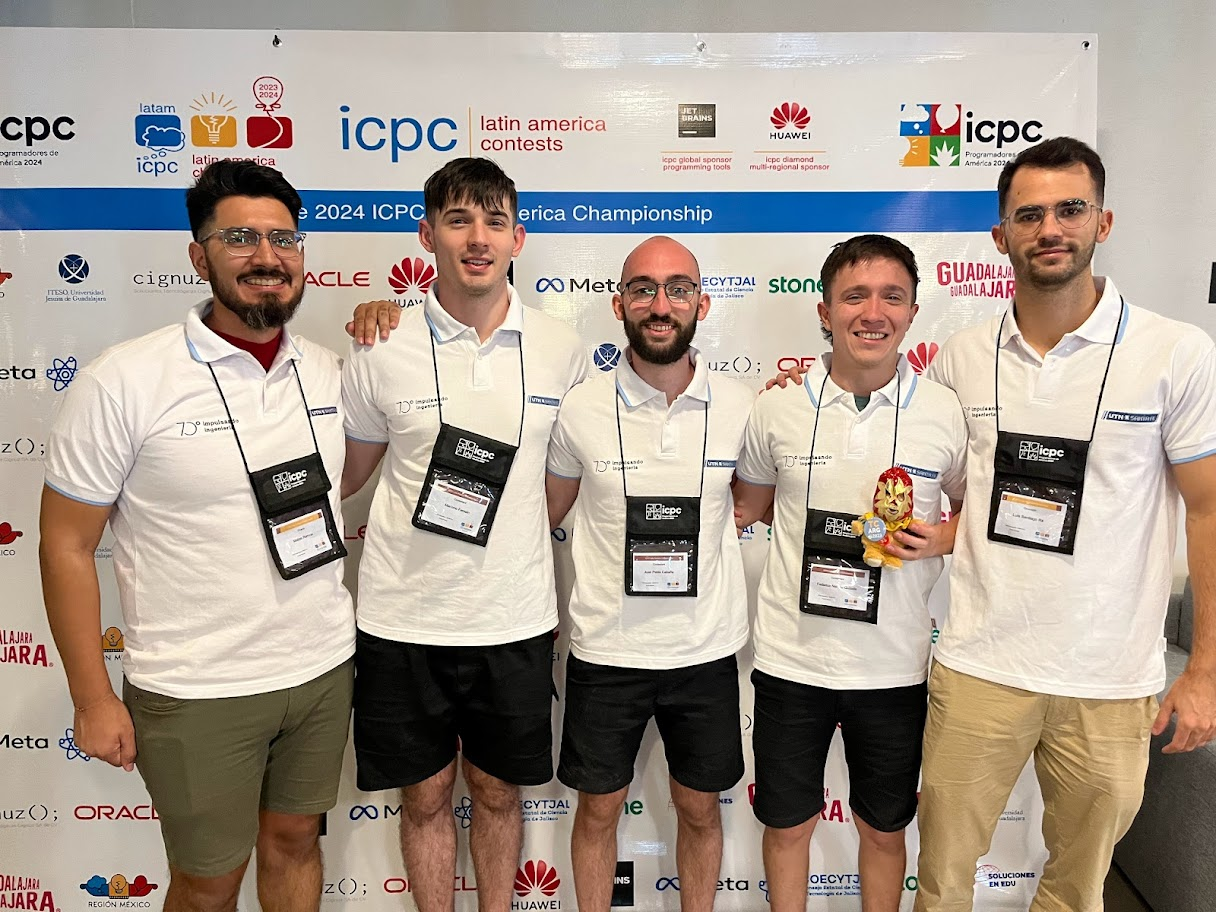
\includegraphics[width=\linewidth]{fotos/mexico.jpg} \\
        \centering \small Fruta Fresca (México '24)
      \end{minipage}
      \\[1cm]  % Vertical space between rows
      \begin{minipage}{0.35\textwidth}
        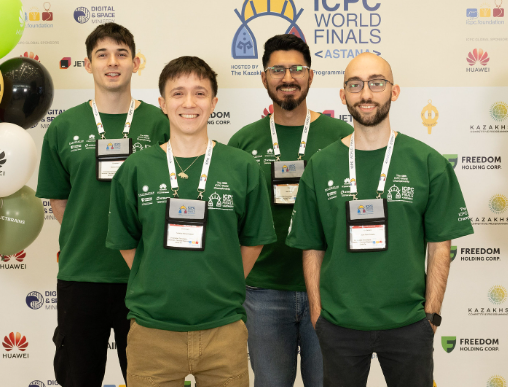
\includegraphics[width=\linewidth]{fotos/kazajistan.png} \\
        \centering \scriptsize \makebox[0.95\linewidth]{Fruta~Fresca~(Kazajistán~'24)}
      \end{minipage}
      &
      \begin{minipage}{0.35\textwidth}
        
\includegraphics[width=\linewidth]{fotos/champan.png} \\
        \centering \scriptsize \makebox[0.95\linewidth]{Champán~en~Lata~(Brasil~'25)}
      \end{minipage}
    \end{tabular}
  \end{center}

\end{frame}



\section{¿Qué es un problema?}

\begin{frame}
  \frametitle{¿Qué es un problema?}

  \textbf{Problema de ejemplo:}
  
  Juan tiene $0 \leq X \leq 90$ manzanas, y quiere repartirlas entre $0 \leq Y \leq 10$ amigos. \\
  Suponiendo que quiere maximizar la cantidad de manzanas que reparte, y que todos reciban la misma cantidad,\\
  ¿cuántas manzanas recibiría cada uno?

  \textbf{Input:}

  2 \\
  15 2 \\
  17 5 \\

  \textbf{Output:}

  7 \\
  5 \\

\end{frame}


\section{Operaciones}

\begin{frame}
  \frametitle{Operaciones}

  \textbf{¿Cuántas operaciones entran en tiempo?}

  Podemos dividir en tres secciones:
  
  \begin{itemize}
    \item \textcolor{green!60!black}{\textbf{$\leq 10^8$ operaciones}}: Siempre entran en 1 segundo.
    \item \textcolor{orange!90!black}{\textbf{Entre $10^8$ y $10^9$ operaciones}}: Puede funcionar, dependerá principalmente de qué hace cada operación.
    \item \textcolor{red}{\textbf{$> 10^9$ operaciones}}: \textbf{PELIGRO}: casi siempre lleva a \texttt{TIME LIMIT}.
  \end{itemize}

\end{frame}

\begin{frame}
  \frametitle{Límites y Overflow}

  \textbf{Los tipos de datos tienen sus límites también:}

  \begin{itemize}
    \item \texttt{int} $\Rightarrow$ desde $-2^{31}$ hasta $2^{31}-1$ ($\approx \pm 2 \cdot 10^{9}$)..
    \item \texttt{long long} $\Rightarrow$ desde $-2^{63}$ hasta $2^{63}-1$ ($\approx \pm 9 \cdot 10^{18}$).
  \end{itemize}

  \vspace{0.3cm}
  \textbf{Al superar esos límites, llegamos al famoso \textcolor{red}{\texttt{OVERFLOW}}.}

\end{frame}


\begin{frame}
  \frametitle{¿Cómo evitar el overflow?}

  \textbf{El overflow es un error \textcolor{red}{MUY COMÚN}.}

  \vspace{0.2cm}
  El uso de \textbf{aritmética modular} (A.K.A. operaciones MOD) es fundamental:  

  \begin{itemize}
    \item \texttt{\%} (MOD): devuelve el resto de una división.
    \item \texttt{ADD mod}: $(a + b) \bmod m$
    \item \texttt{SUB mod}: $(((a - b) \bmod m) + m ) \bmod m$
    \item \texttt{MUL mod}: $(a \cdot b) \bmod m$
  \end{itemize}

  \vspace{0.2cm}
  \textbf{Recomendaciones:}
  \begin{itemize}
    \item Usar tipos de 64 bits: \texttt{long long} en C++.
    \item Es mejor usar \texttt{MOD} de más que de menos.
  \end{itemize}

\end{frame}



\section{Estructuras útiles}


\begin{frame}
  \frametitle{Operaciones útiles}

  \textbf{Operaciones comunes:}
  \begin{itemize}
    \item \texttt{sort(v.begin(), v.end(), comparador);}
    \item 
    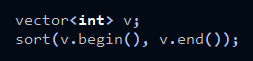
\includegraphics[width=0.4\textwidth]{fotos/sort.png}
    \item \texttt{lower\_bound(v.begin(), v.end(), x);} (requiere orden)
    \item \texttt{set.lower\_bound(x);} (asi se usa en sets)
    \item \texttt{upper\_bound();}
  \end{itemize}
\end{frame}


\begin{frame}
  
  \frametitle{Estructuras importantes}
  Hay algunas estructuras que son \textbf{muy importantes}:
  \begin{itemize}
    \item \texttt{vector}
    \item \texttt{queue}
    \item \texttt{deque}
    \item \texttt{set}
    \item \texttt{map}
  \end{itemize}
\end{frame}



\begin{frame}
  \frametitle{Vector}
  \begin{itemize}
    \item \texttt{vector<T>} en C++, con \texttt{push\_back} y \texttt{pop\_back}
    \item \texttt{ArrayList<T>} en Java, con \texttt{add} y \texttt{remove(list.size()-1)}
    \item \texttt{list} en Python, con \texttt{append} y \texttt{pop}
    \item Acceso con \texttt{v[pos]} o \texttt{v.get(pos)}
    \item Todas estas operaciones son \textbf{O(1)}
  \end{itemize}
\end{frame}

\begin{frame}
  \frametitle{Queue}
  \begin{itemize}
    \item \texttt{queue<T>} en C++, con \texttt{push}, \texttt{front}, \texttt{pop}
    \item \texttt{ArrayDeque<T>} en Java, con \texttt{add}, \texttt{getFirst}, \texttt{remove}
    \item \texttt{collections.deque} en Python, con \texttt{append}, \texttt{deque[0]}, \texttt{popleft}
    \item Se comporta como una cola (FIFO)
    \item Operaciones en \textbf{O(1)}
  \end{itemize}
\end{frame}

\begin{frame}
  \frametitle{Deque}
  \begin{itemize}
    \item \texttt{deque<T>} en C++, con \texttt{push\_front}, \texttt{push\_back}, \texttt{pop\_front}, \texttt{pop\_back}
    \item \texttt{ArrayDeque<T>} en Java, con \texttt{addFirst}, \texttt{addLast}, \texttt{removeFirst}, \texttt{removeLast}
    \item \texttt{collections.deque} en Python, con \texttt{appendleft}, \texttt{append}, \texttt{popleft}, \texttt{pop}
    \item Acceso en \textbf{O(1)}
    \item Todas las operaciones anteriores son también \textbf{O(1)}
  \end{itemize}
\end{frame}

\begin{frame}
  \frametitle{Set}
  \begin{itemize}
    \item \texttt{set<T>} en C++
    \item \texttt{TreeSet<T>} en Java
    \item En Python no hay un equivalente ordenado nativo
    \item Mantiene elementos \textbf{únicos y ordenados}
    \item Permite insertar, borrar, consultar existencia, \texttt{lower\_bound}, \texttt{upper\_bound}
    \item Todas en \textbf{O(log N)}
    \item Variantes:
    \begin{itemize}
      \item \texttt{unordered\_set} (C++) / \texttt{HashSet} (Java): O(1) amortizado
      \item \texttt{multiset}: permite elementos repetidos
    \end{itemize}
  \end{itemize}
\end{frame}

\begin{frame}
  \frametitle{Map}
  \begin{itemize}
    \item \texttt{map<K, V>} en C++
    \item \texttt{TreeMap<K, V>} en Java
    \item En Python: \texttt{collections.OrderedDict} (aproximado)
    \item Mantiene pares \textbf{clave → valor}
    \item Acceder, insertar, borrar en \textbf{O(log N)}
    \item Variante: \texttt{unordered\_map} (hash, O(1) amortizado)
  \end{itemize}
\end{frame}


\section{Entrada y salida}

\begin{frame}{Entrada y salida en C++}
  \textbf{Forma elegante de entrada/salida:}
  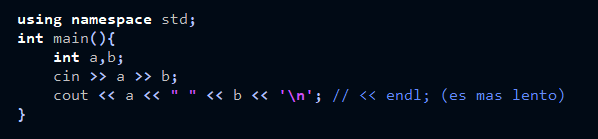
\includegraphics[width=0.8\textwidth,keepaspectratio]{fotos/cin.png}

  \vspace{0.2cm}
  Leer y escribir consume tiempo, por lo tanto hay que tener cuidado.
\end{frame}

\begin{frame}[fragile]{Acelerando entrada/salida}

  \textbf{Recomendaciones en C++:}
  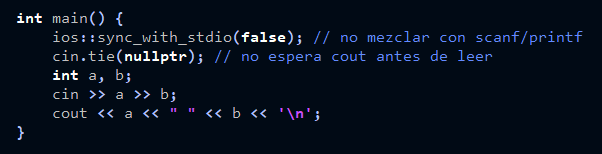
\includegraphics[width=0.8\textwidth,keepaspectratio]{fotos/fastcin.png}
\end{frame}

\section{Consejos personales}

\begin{frame}[fragile]{Consejos personales}
  \begin{itemize}
  \item  Usar una tablita para anotar ideas por problema
  \end{itemize}

  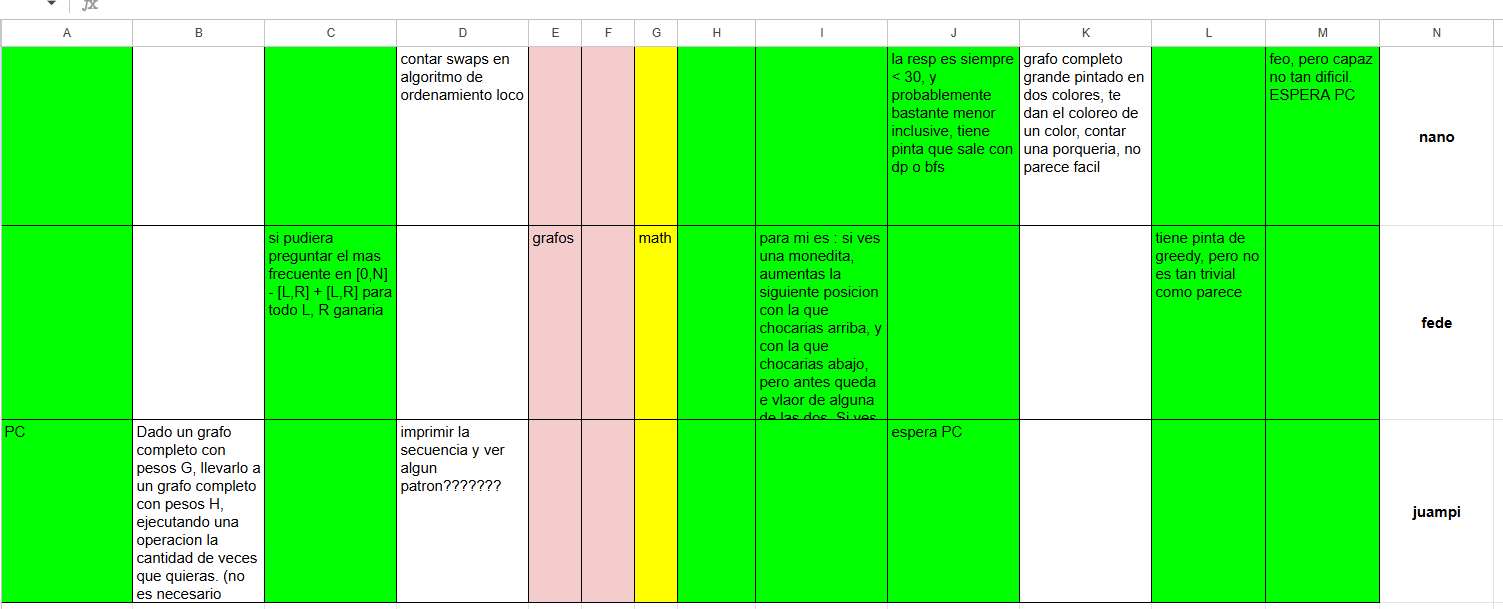
\includegraphics[width=1\textwidth,keepaspectratio]{fotos/tablita.png}

  \begin{itemize}
  \item Aprovechar simulaciones para mejorar la dinámica
  \item Mantener una buena comunicación con el equipo
  \end{itemize}

\end{frame}


\begin{frame}[fragile]{Consejos personales}
  \begin{itemize}
  \item Tener un template útil y propio
  \end{itemize}
  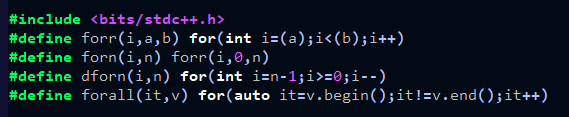
\includegraphics[width=0.8\textwidth,keepaspectratio]{fotos/template.png}

  \begin{itemize}
  \item Acostumbrarse a usar un notebook
  
  \item Aprender a estimar tiempos 
  \item Leer editoriales → entender el \textbf{cómo}, no solo el código
  \item Usar IA como herramienta, no como solución
  \end{itemize}
\end{frame}


\begin{frame}[fragile]{Consejos personales}
  \begin{itemize}
  \item \textbf{UPSOLVEAR}, esa es la clave
  \end{itemize}
  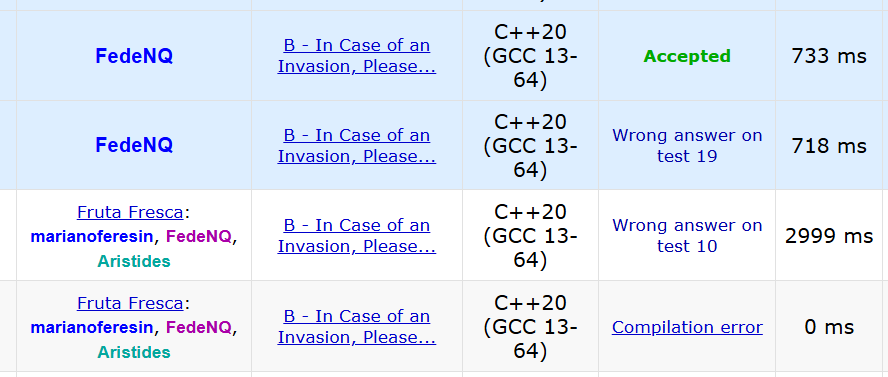
\includegraphics[width=1\textwidth,keepaspectratio]{fotos/uplsoving.png}
  
\end{frame}


\begin{frame}[fragile]{Consejos personales}
  \begin{itemize}
  \item No quedarse con un solo problema, leer otros.
  \item Intentar resolver casos mas simples, ver como mejorar la solucion.
  \item Disfrutar, tanto las competencias como los entrenamientos
  \end{itemize}
  
\end{frame}

\begin{frame}[fragile]{Consejos personales}

  Fin!!
  Gracias por asistir! 

  Muchos éxitos en la compe de hoy
  
\end{frame}

\end{document}